\documentclass{article}

\usepackage[utf8]{inputenc}
% Use nameref to cite supporting information files (see Supporting Information section for more info)
\usepackage{nameref,hyperref}
% amsmath and amssymb packages, useful for mathematical formulas and symbols
\usepackage{amsmath,amssymb}
% useful for consistent display and control of units of measurement
\usepackage{siunitx}
% figures!
\usepackage{graphicx}
% for including TODO notes
\usepackage{todonotes}
% snyntax highlighting for code
\usepackage{minted}
% manually set margins
\usepackage{geometry}[margins=1in]

\title{Analysis and Ethical Design of Terrain Park Jumps for Snow Sports}
\author{Jason K. Moore, Bryn Cloud, Mont Hubbard, Christopher Brown}
\date{\today}

\begin{document}

\maketitle

\begin{abstract}
  Terrain parks now exist at almost all US snow sport resorts. For several
  decades, epidemiological evidence shows increased injuries correlate with
  terrain park use. Injury risk could be reduced through analytical engineering
  design of jump profiles to control the equivalent fall height, i.e., energy
  dissipated on impact when landing. The ski industry and their insurance
  companies are resisting making terrain park jumps safer in this way. We
  discuss two case studies illustrating that large equivalent fall heights play
  significant roles in traumatic injuries in terrain park jumps. As a remedy,
  we provide an accessible online tool for terrain park builders, both to
  evaluate safety of existing jumps by calculating their impact danger and to
  design jump profile shapes that control equivalent fall heights and thereby
  reduce the risk of injury.
\end{abstract}

\section{Introduction}
%
When a falling person impacts a fixed surface, there is risk of injury. Greater
impact velocity normal to the surface causes greater injury, due to increased
kinetic energy that must be dissipated on impact. A common surrogate for
measuring impact energy is ``equivalent fall height'', a conceptually simple
and familiar interpretation of impact danger used in a variety of safety
standards around the world, from construction~\cite{OSHA2021} to children's
playground equipment~\cite{Chalmers1996}. The equivalent fall height of ski and
snowboard terrain park jumps can be calculated~\cite{McNeil2012} if the Cartesian coordinates of
the jump profile are known including  the starting point, take off and
landing hill along the jumper's path. Controlling energy
dissipation in the human body, and hence equivalent fall height in terrain
park jumps, is paramount to safe design methods to reduce likelihood and
severity of injury.

This paper discusses societal costs of increasing terrain park injuries and
focuses on two case studies that illustrate the danger, if equivalent fall
height is not controlled. We then present a user-friendly web application for
calculating equivalent fall height of existing or planned jumps. We see this
application as a part of the solution to reducing injuries in terrain park
jumps. Jump builders may use it to reduce the risk of injuries in their
resorts.

\subsection{History}
%
Terrain park jumps are not a new addition to snow sports resorts. Their gradual
introduction in the 1980's was tied to increased interest in aerial maneuvers
and extreme sports participation. Growth accelerated and has continued.  Today
nearly 95\% of US ski resorts include terrain parks. Unfortunately, this
ubiquity is correlated to injury increases.  Two early longitudinal studies  in
the 1980's and early 1990's~\cite{Diebert1998,Furrer1995} had already found
significant increases in head injuries and concussions. The Consumer Product
Safety Commission~\cite{CPSC1999} learned that between 1993 and 1997 head injuries accounted
for a majority of skiing
and snowboarding deaths. An early review~\cite{Koehle2002} noted that "[S]eventy-seven
percent of spinal injuries~\cite{Tarazi1999} and 30\% of head
injuries~\cite{Fukada2001}
in snowboarding were a result of jumps." Jackson et al.~\cite{Jackson2004}
determined that by 2004 snow skiing had replaced football as the second leading
cause of serious head and spinal cord injuries in the US.

These early increasing injury assessments persisted. According to
\cite{Russell2014}, "between 5\% and 27\% of skiing and snowboarding injuries
occur[red] in terrain parks \cite{Bridges2003, Goulet2007,  Moffat2009,
Greve2009, Brooks2010,and Ruedl2013}".  Incredibly, at the first Winter Youth
Olympic Games more than a third of all snowboard half-pipe and slope-style
competitors became injured \cite{Ruedl2012}. Epidemiological research
continues to show \cite{Carus2016,Audet2019, Hosaka2020} that injuries on
terrain park jumps are both more likely and more severe than those on normal
slopes. Audet et. al~\cite{Audet2019} states  there is strong evidence that
skiing or snowboarding in a terrain park is a risk factor for head, neck,
back, and severe injuries. Hosaka et. al~\cite{Hosaka2020} concludes that
jumping is one of the main causes for serious spinal injuries, regardless of
skill level, and suggests that, because the incidence of spinal injuries has
not decreased over time, ski resorts and the ski industry should focus on
designing fail-safe jump features to minimize the risk of serious spinal
injury.  Similar suggestions have repeatedly been made in peer-reviewed
literature for more than a decade
\cite{Hubbard2009,Swedberg2012,McNeil2012,McNeil2012a,McNeil2015,Hubbard2015,
Levy2015,Petrone2017,Moore2018}.

\section{Equivalent Fall Height}
%
\emph{Equivalent fall height} is a common proxy measure for impact danger by
industry in safety standards~\cite{Hubbard2012}, the kinetic energy that must
be dissipated on impact from a given height. On the earth's surface this energy
is given by the well known equation $mgh$ and is equal to the linear kinetic
energy available to injure a person in a non-rotating fall. The ability of this
energy to injure can be reduced by controlling impact circumstances, e.g.
impact cushioning, body orientation, body configuration and active body motion;
however this energy must be dissipated. Larger equivalent fall heights require
more elaborate protection measures to reduce injury.

Equivalent fall height is a particularly useful measure of danger due to its
interpretability by lay people. People have an intuitive danger sense when
faced with potential falls from large heights and they have strong common sense
for relating fall height to likelihood of injury due to experience with their
own and others' falls. For example, we have a sense of the danger associated
with falling from building stories of increasing magnitude. Ground floor falls
are on the order of 2.6~\si{\meter}, second story are 5.1~\si{\meter}, third
story 8.8~\si{\meter}, and so on~\cite{Vish2005}. OSHA requires fall protection
for fall heights greater than 1.2~\si{\meter} for general workplace
safety~\todo{OSHA1994} and the FAA's safety regulations for safe parachuting
landings is a 3~\si{\meter} fall height~\todo{need citation}.  Chalmers et
al.~\cite{Chalmers1996} pushes for 1.5~\si{\meter} maximum fall heights for
playground equipment. As for skiing, the standards for the Olympic traditional
Nordic ski jumping call for equivalent fall heights of
0.46~\si{\meter}~\todo{need citation}.

The equivalent fall height $h$ of an object is formally defined as
%
%\begin{align}
  
%  \label{eq:efh_general}
%\end{align}
%
where $v$ is the impact velocity of the object and $g$ is the acceleration due
to gravity. This definition results from equating the kinetic energy of an
object moving at velocity $v$ at impact with the potential energy of the same
object at a height $h$ above the ground.

Using Equation~\ref{eq:efh_general} as a starting point, the equivalent fall
height $h$ can be determined for any landing surface one impacts after a jump
flight trajectory~\cite{Hubbard2012}. The resulting equation, neglecting air
drag here for simplicity, is
%
\begin{align}
  h = \left[\frac{x^2}{4(x\tan\theta_T - y)\cos^{2}\theta_T} -
    y\right]\sin^{2}\left[\tan^{-1}\left(\frac{2y}{x}- \tan\theta_T\right) - \tan^{-1}\frac{dy}{dx}\right]
  \label{eq:efh}
\end{align}

This expression is  a function of only four variables: takeoff angle
$\theta_T$, impact coordinates $(x,y)$ on the landing surface, and the slope of
the landing surface $\frac{dy}{dx}$. It is important to note that this surface
is not a function of takeoff speed. To analyze a jump, it is sufficient to
measure the Cartesian coordinates of the landing surface along the jumper's
flight path and the takeoff angle. Slopes $\frac{dy}{dx}$ are computed
numerically from the measured coordinates $(x,y)$.  LET'S EXPLAIN WHY SPEED CAN
BE IGNORED.

\section{Case Studies}
%
Below we present two case studies from court proceedings in the United States.
In these cases juries ruled in favor of injured plaintiffs, judging that
neglect in jump design and construction contributed significantly to their
injuries. Simulation results below assume skier mass, frontal area, and drag
coefficient of 75~\si{\kg}, 0.34~\si{\meter\squared}, and 0.821, respectively.

\subsection{Vine v. Bear Valley}
%
In April 2000, Ms.~Vine's lower spine was injured when she fell on a jump at
Bear Valley Ski Resort in California. The jump shape was a ``tabletop'', a
common form of terrain park jump.  The builder's intent is that jumpers
completely clear the table, landing on the down-slope near the so-called
``sweet spot'', but Vine landed short of the knuckle (end of the tabletop). The
upper panel of Fig.~\ref{fig:vine-v-bear-valley} shows the jump surface (solid
black) based on  accident investigation measurements. This tabletop, which
would typically be flat and horizontal, was instead concave, compounding the
danger of a short landing.  At the 11~\si{\meter} actual measured horizontal
landing distance from the takeoff point, the surface was sloped upwards
approximately 5\si{\degree}.  The surface shape emphasizes the detrimental
effect of not aligning more closely the surface tangent with the jumper flight
path at impact.
%
\begin{figure}
  \centering
  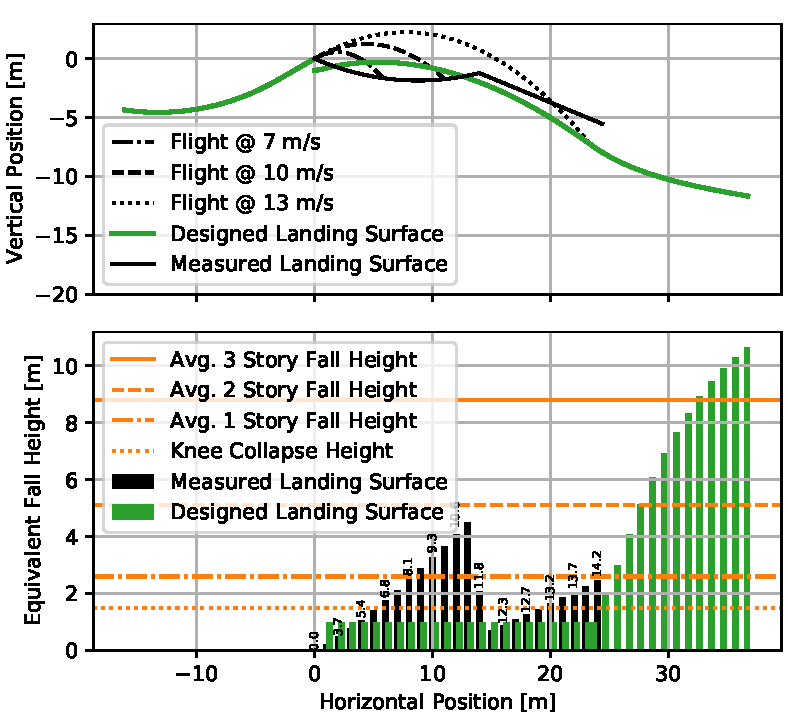
\includegraphics[width=5.25in]{figures/vine-v-bear-valley.pdf}
  \caption{\textbf{Bear Valley jump compared to possible safer design}
  a) Measured landing surface (solid black) and jumper flight paths (intermittent
  black) from 30\si{\degree} takeoff angle. The
  13~\si{\meter\per\second} takeoff speed is used as the design speed for a comparison 
  jump (solid green) designed to have constant equivalent fall height of 1~\si{\meter}. 
  b) Lower panel shows equivalent fall height for both jumps
  in corresponding colors at 1~\si{\meter} intervals. Numbers above 
  vertical bars indicate takeoff speed required
  to land at that location. Orange lines indicate relatable fall heights.}
  \label{fig:vine-v-bear-valley}
\end{figure}

~\todo{ remove data in Fig for distances greater than 28 m.   Mont}
The lower panel plots equivalent fall height at different landing
locations. It is clear that just short of the knuckle, the
equivalent fall height is highest. At a landing distance of 12 meters, Vine's fall height would have been
about 4 meters, equivalent to falling from between one and two storeys \cite{Vish2005}.
Vine's body had also
rotated backward in flight. She landed on her lower spine and was paralyzed as a result
of the nearly two story fall. A lower equivalent fall height would have decreased the
possibility of spinal injury, due to the lower impact forces.

%On this jump, if the jumper's landing position is less than 5~\si{\meter} or
%greater than 18~\si{\meter} ~\todo{Greater than 18m from where? the takeoff
%point? -Bryn} the equivalent fall height is less than that which causes knee
%collapse~\cite{Minetti1998}, but in the range that jumpers are more likely to
%land the equivalent fall height can become quite dangerous, especially if the
%jumper rotates for a fall on their head as Ms.~Vine did. If a jumper lands in
%the area at the end of the concave tabletop, it is equivalent to falling out of
%a second story window. 

In contrast, a landing surface designed to have a constant equivalent fall
height can be created with a similar amount of construction costs that would
reduce the fall height.  The green jump profile in the upper panel of
Figure~\ref{fig:vine-v-bear-valley} shows a possible jump design,
~\cite{Levy2015}, of similar size with similar flight times that ensures a
constant equivalent fall height everywhere of 1~\si{\meter}.  The convex shape
of this jump is interestingly close to what one would get if the original
tabletop were inverted, showing how the convex nature of the jump shape is
critically important to control equivalent fall height. A jump of this design
would have lowered impact forces for any orientation landing at any possible
landing location. In 2002, the jury ruled in favor of Ms.~Vine, agreeing that
Bear Valley was responsible for designing safer jumps~\cite{Alvarado2002}.

\subsection{Salvini v. Ski Lifts Inc.}
%
In 2004, Mr.~Salvini attempted a table-top jump on skis in the terrain park of
the The Summit at Snoqualmie ski resort, in Washington state.  Salvini overshot
the intended landing location even while traveling at expected skiing speeds,
rotated backward during flight and landed on his back, ultimately causing
quadriplegia. At his landing location the equivalent fall height was over 10
meters, approximately a 4-story fall.  Figure~\ref{fig:salvini-v-snoqualmie}
shows the jump profile in a solid black line based on measurements from the
accident investigation.  For takeoff speeds greater than
13~\si{\meter\per\second} (47~\si{\kilo\meter\per\hour}), the lower panel
shows, also in black, that the equivalent fall height is greater than 8 meters
and grows linearly with larger takeoff speeds. Severe injury is almost certain
from falls this high, especially so if landing in a way that causes undue
forces to the spine, as in this case.

The green curve in the upper panel is the jump profile designed to have a
1~\si{\meter} equivalent fall height for all speeds below
17~\si{\meter\per\second}. This profile requires significantly more snow than
the measured jump but alleviates the dangerous impacts possible in the measured
jump.

This jump highlights how extreme the equivalent fall height can be if the jump
is not designed properly and ethically. Few recreational skiers will jump out
of a four story window, snow landing or not. The likelihood of injury is quite
clear and our internal altimeter tells us so. However, our internal altimeters
cannot sense potential risks until we have left the takeoff are in the air.
%

\begin{figure}
  \centering
  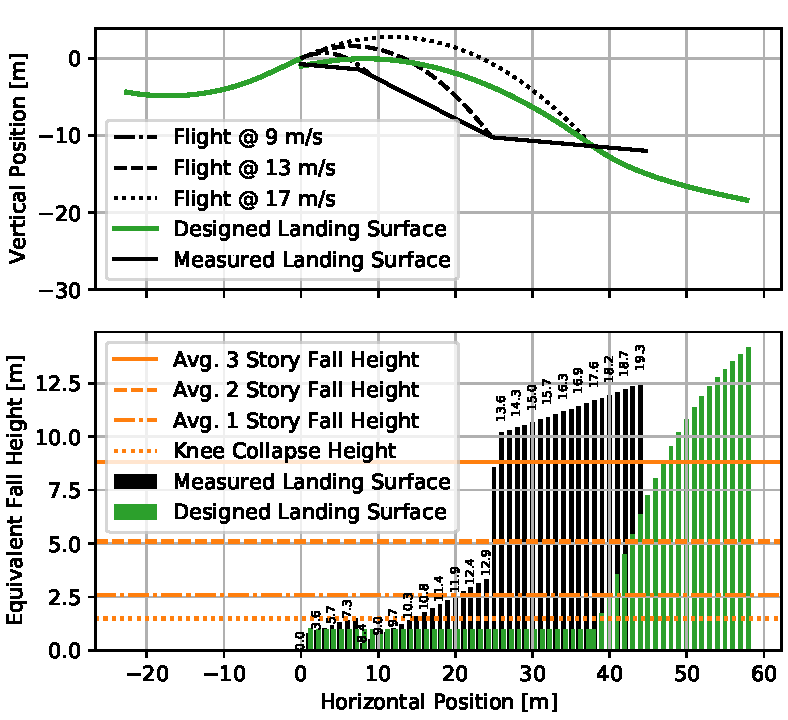
\includegraphics[width=5.25in]{figures/salvini-v-snoqualmie.pdf}
  \caption{\textbf{Snoqualmie jump compared to possible safer design}
  a) Measured landing surface (solid black) and jumper flight paths (intermittent
  black) for 25~\si{\degree} takeoff angle. The
  17~\si{\meter\per\second} takeoff speed is used as the design speed for a comparison
  jump (solid green) designed to have constant equivalent fall height of 1~\si{\meter}.
  b) Lower panel shows equivalent fall height for both jumps
  in corresponding colors at 1~\si{\meter} intervals. Numbers above
  vertical bars indicate takeoff speed required
  to land at that location. Orange lines indicate relatable fall heights.}
  \label{fig:salvini-v-snoqualmie}
\end{figure}

\section{Moral Imperative}
%
Employing engineering ethically to reduce the risk of injury on fabricated
terrain park jumps, motivates this work. Engineering analysis and design, based
on the laws of mechanics can be used shape terrain park jumps to limit
equivalent fall heights. These laws go back centuries to Issac Newton and
Émilie du Châtelet, \cite{Zinsser2007}. These are introduced in high school physics and
are fundamental in engineering education. Our motivation complies with the
first canon of engineering ethics: ``Hold paramount the safety, health and
welfare of the public''~\cite{NSPE2019}. In the context of snow sport safety,
the first canon compels engineers to direct their technical expertise to
protecting snow sport participants from injuries. No one can rationally argue
that reducing equivalent fall height would cause an increased likelihood of
injury and, if shaping designed jump landing surfaces is no more laborious than
shaping non-designed surfaces, there can be no reason not to attempt to control
for equivalent fall height. Then what explains the reluctance of the skiing
industry and their insurance companies to adopt such design methods?

People unfamiliar with the legal and insurance systems in the USA may fail to
appreciate that technical literature is often corrupted in legal defense of
unsafe practices and protecting corporate assets. Peer-reviewed technical
literature is used to support testimony in U.S. lawsuits. Both plaintiffs and
defendants hire their own experts to testify and authors of technical papers
can make money by testifying. When this testimony is for the defense, the
testimony can result in denying compensation for injuries, and serve to prolong
unsafe practices. Rarely do experts report conflicts of interest in their
papers and presentations, or when they organize and chair meetings or edit
publications. Financial support for publications used by expert witnesses can
be routed through consulting companies to pretend some deniability of conflicts
of interest in their papers. Sadly, this is deceitful, self-serving, and
unethical, because it ignores the first canon of engineering ethics. It should
be argued that, if someone ignores engineering ethics, they are not acting as
engineers, and what they are doing cannot be considered engineering.

Designing jumps to limit equivalent fall height and reduce the risk of injuries
is based on well-known, well-established, centuries-old physics. The concept
that designing jumps, to limit equivalent fall height and control energy
dissipation, can reduce injury risk, is irrefutable. Said another way, impact
energy in a jump landing could be set a walking speed. This speed a magnitude
that evolution has apparently guaranteed not to cause a walker serious injury.
Yet, these jumps are built such that injury from impact is much more likely. To
counter this solid, fundamental, scientific concept defense experts introduce
confounding factors are that serve to cloud and confuse the basic issues.
Consider three examples of papers co-authored by well-known skiing industry
defense experts who have testified for the ski industry and their insurance
companies.

Shealy et. al~\cite{Shealy2010} conducted an experimental study which attempts
to test the hypothesis that takeoff speed is a predictor of the distance from a
take-off to a jump landing. They indicate that a series of jumpers who use a
terrain park jump land within a narrow region, which is reasonable once it is
noted that the jumpers' takeoff speeds did not vary much either, i.e. no
attempt was made to assess a reasonable range of their independent variable.
The authors state both that there is ``no statistically significant
relationship between takeoff speed and the distance traveled'' and that
``takeoff speed is not a dominant or controlling factor (in how far a jumper
travels)''. These results should lead the careful researcher to question their
experimental design and analysis methods, just as a high school physics student
should if their an object in their lab experiment does not fall with an
acceleration close to 9.8~\si{\meter\per\second\squared}.

Shealy et. al~\cite{Shealy2015} claim that catastrophic and fatal injury rates
at US snow resorts have not changed, even though terrain parks (and thus likely
jumping) have increased over time. The statistical model in this study by
Shealy et al. 2015 was expressly designed such that only passage of time was
used as an explanatory variable for incident rates. The authors do not report
absolute numbers of fatalities and injuries, only incident rates, which provide
a more favorable view for the ski industry and their risk assessment. They use
weighting factors which they don not disclose in order to harmonize data over
time. One should question what these weightings are.  Data and robust modern
statistical methods exist for testing their stated hypothesis. We can only
speculate as to why those may have not been used for this analysis. Drawing
their final conclusion, that addition of terrain parks mitigates risks, is
quite a stretch, given the data and debatable analysis.When it comes to health
and safety of the public, society is also interested in reducing or eliminating
the absolute numbers. This is especially true for activities in which the risk
of catastrophic life-changing or fatal injuries can be mitigated by ethical
engineering designs, and therefore are not be inherent to the sport.
%
In an article on landing positions~\cite{Scher2015}, Scher et. al show that
body orientation at impact can cause dangerous cervical spine loads. They
report on effects of equivalent fall height but only test heights from
\SIrange{0.23}{1.52}{\meter}, both committing a similar fault as done in
\cite{Shealy2010} restricting the range of their independent variable
inappropriately, and not testing fall heights that are known to have caused
severe injury. Yet the authors purport that equivalent fall height has no
appreciable effect on injury. The title of this paper, ``Terrain Park Jump
Design: Would Limiting Equivalent Fall Height Reduce Spinal Injuries?'' implies
that the authors may believe falling on ones head from greater and greater
heights may \emph{not} cause greater injuries. It is not clear why one might
propose such a hypothesis in the first place.

The first two studies do a poor job of isolating variables, and apparently were
not intended to, and the third suffers from restriction of equivalent fall
height range. But most importantly, and quite noticeably, none of these papers
are written with the intent to reduce injury rates. No ways are suggested in
which their findings could be used to promote the safety, health, and welfare
of the public. What these papers have done, is attempt to muddy the waters
regarding the fact that impacting a surface at a lower velocity is safer. This
strategy of introducing bogus science is well know in litigation in the U.S..
For example the same strategy was used to defend the tobacco industry
[Merchants of Doubt, Naomi Oreskas and Erik M. Conway, Bloomsbury, 2010].

Testifying for an injured plaintiff, or to defend corporations, in injury
cases, are not equivalent actions ethically. Authoring papers with no intent on
improving safety and reducing injuries is unethical. One attempts to address
problems that cause injuries, holding paramount the safety health and welfare
of the public. The other attempts to defend the practices that might have
contributed to the injury, in order to limit financial losses of insurance
companies. The proverbial two sides to every question do not exist in science
and engineering.

Poorly executed experiments in snow sports or elsewhere, no matter how
expensive and sophisticated the instrumentation, cannot disprove the
fundamental laws of  mechanics. If statistics or experimental results do seem
in conflict with predictions from classical mechanics, then there is likely a
problem with the statistical or experimental design or its interpretation, and
not with the mechanics itself. Defending practices that lead to injuries at the
service of protecting corporate assets can prolong these practices, which can
lead to further injuries, clearly violating the first canon of engineering
ethics.

\section{What Can Be Done?}
%
Assessing and reshaping existing jumps for dangerous equivalent fall heights
should be an easy way for ski resorts to reduce the danger of their terrain
park jumps. Accurate enough measurements of an existing slope can be done with
simple tools, e.g. a tape measure and a digital level, and only takes a short
amount of time per jump, see Appendix~\ref{sec:jump-shape-measurement}.  The
calculation and visualization of the equivalent fall height from these
measurements can take some time if manually done. A program for calculating
equivalent  fall heights from a hill profile is to be available an online,
freely accessible, and user friendly web application that makes the calculation
and visualization step almost instantaneous for the terrain park builder. With
the tool described in the next section, terrain park builders can easily add
this safety assessment to their toolbox, even using it from a smartphone while
in the field. There is no reason that this basic assessment should not be part
of the jump construction process. The laws of nature clearly tell us that
designing jumps with lower equivalent fall heights will have a positive
probability in reducing injuries.  The only ethical decision is to adopt these
methods; as saving even one person from a life of paralysis must be worth the
minor inconvenience of shaping jumps using the rules in \cite{Levy2015}.

Standards - ASTM F27
Struggle to write ski binding adjustment standards
Modified scope to avoid writing standards on snow surfaces

Insurance and risk 

\subsection{Software and Online Access}
%
Software has been for designing ski jumps with a constant equivalent fall
height~\cite{Moore2018}. The software comprises of a general purpose,
extensible, object oriented software library with tools for 2D skiing
simulation. Using the library code, a web application was developed for
interactive jump design. The web application is designed for a non-technical
end user and usable on a desktop, tablet, or mobile device; any device that
supports a web browser.

We have extended the capabilities of the software in version 1.4.0 for the
purposes of the work described in this paper. New library features were added
that automate the calculation of equivalent fall height for jump profiles
described by a series of Cartesian coordinates.  Additionally, a new
``analysis'' page was added to the web application which allows users to upload
either a comma separated value CSV text file or a Microsoft Excel spreadsheet
file or with the jump profile coordinates. The jump is then analyzed and the
equivalent fall height is displayed graphically for interactive user
manipulation and viewing. Figure~\ref{fig:web-app-screenshot} shows the web
application with one of the case study jumps loaded for analysis.
%
\begin{figure}
  \centering
  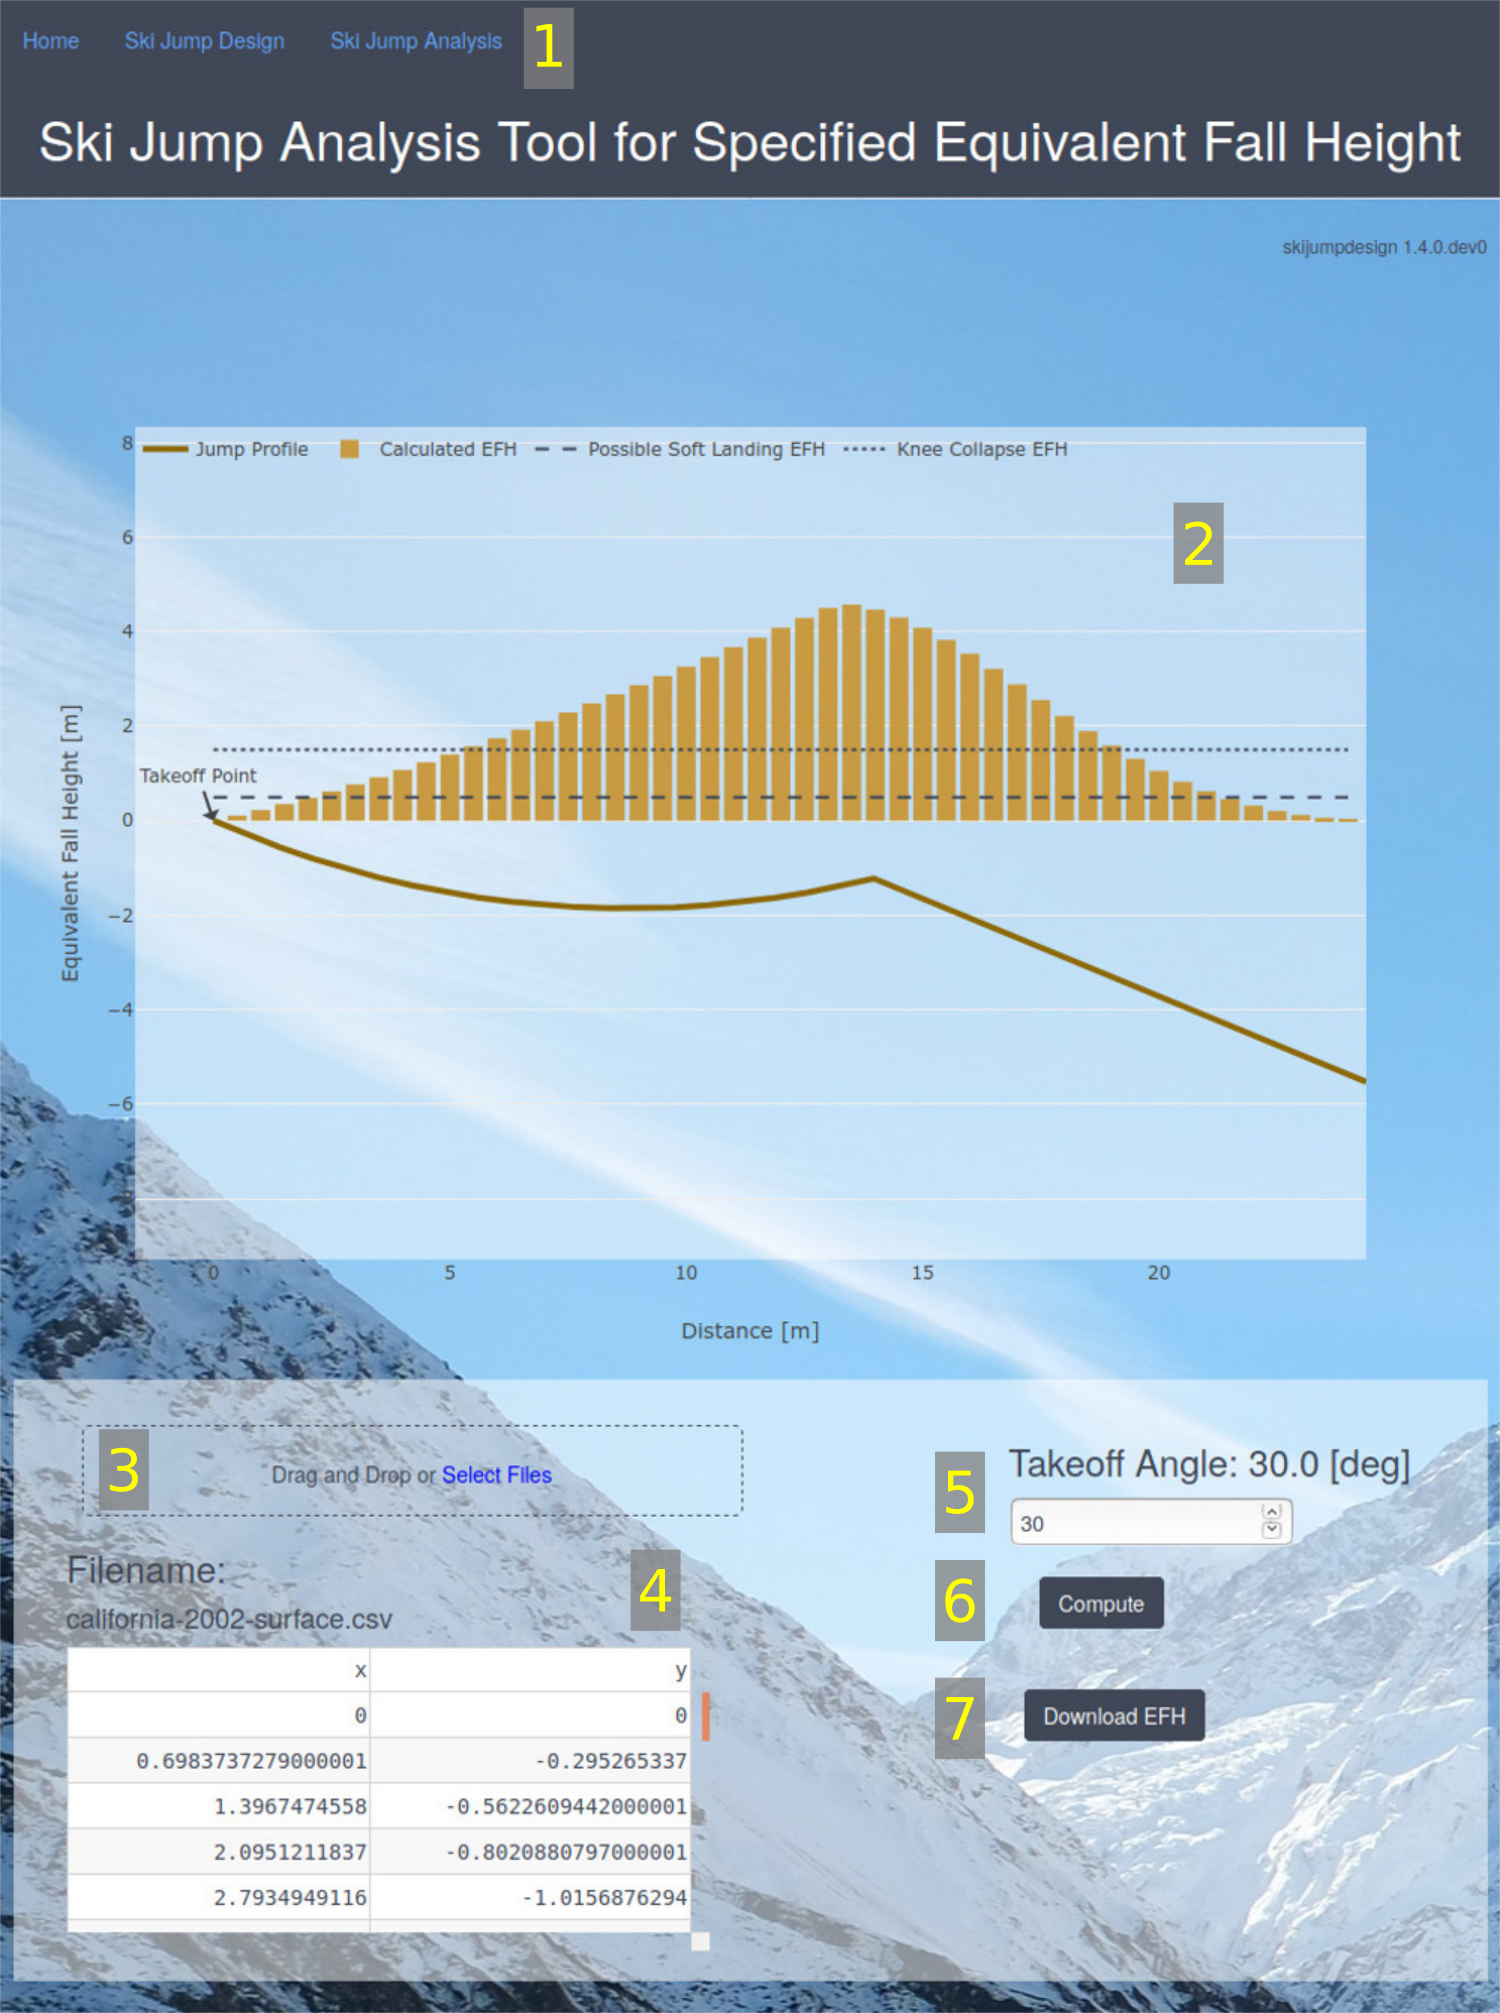
\includegraphics[width=5.00in]{figures/web-app-screenshot.png}
  \caption{\textbf{Screenshot of the web app} To use the app, a user selects
    ``Ski Jump Analysis'' from the primary menu [1], uploads a CSV or XLS file
    by dragging it onto the screen [3], inspects the input data for accuracy in
    the table [4], sets the takeoff angle [5], runs the analysis by pressing
    the ``Compute'' button [6], views the results in the interactive plot [2],
    and downloads the results by pressing the ``Download EFH'' button [7].}
  \label{fig:web-app-screenshot}
\end{figure}

The software is written in Python and directly depends on popular packages
including Cython~\cite{Behnel2011}, matplotlib~\cite{Hunter2007},
NumPy~\cite{Oliphant2006}, pandas~\cite{McKinney2020},
Plotly/Dash~\cite{Plotly2015}, pycvodes~\cite{Dahlgren2018},
SciPy~\cite{Virtanen2020}, SymPy~\cite{Meurer2017}, and xlrd.  The software is
open source and licensed under the MIT redistribution license.  The source code
is available on Gitlab (\url{https://gitlab.com/moorepants/skijumpdesign}) and
PyPi (\url{https://pypi.org/project/skijumpdesign/}. Users can submit bug
reports, feature requests, code improvements, and additions at the Gitlab
repository. The software is documented at
\href{https://skijumpdesign.readthedocs.io}{https://skijumpdesign.readthedocs.io}.
Basic examples of using the library are provided in the appendix.

\section{Conclusion}
%
There are, of course, more factors than jump landing surface shape that
contribute to injuries on terrain park jumps but impact velocity can be easily
controlled with a designed landing surface. There is no evidence to support
that decreasing equivalent fall height increases injuries in falls, only
evidence that injuries can be decreased. Thus there is no reason not to adopt
constant equivalent fall heights of low values for public use jump designs.
Common sense is really all that is needed to believe that falling from higher
heights will increase injury to human bodies regardless of other factors. Any
person that must fall would surely choose to do so from the lowest height.
Constructors of terrain park jumps that are not designed with these facts in
mind are negligent. The safety, health, and welfare of the public involved in
this sport should be held paramount.

\bibliographystyle{unsrt}
\bibliography{references}


\appendix

\section{Example software library use}
%
This closed form equations are useful for understanding the fundamental
relationship of equivalent fall height to the landing surface and well predict
these values for small jumps but other factors may be useful to include in the
model. For example, jumpers are subject to aerodynamic drag and this is not
negligible for larger jumps. If drag is included there is no closed form
solution for the equivalent fall height, but the equivalent fall height can be
computed through iterative simulation~\cite{Levy2015}. The jumper's flight path
is found by integrating the flight equations of motion at various takeoff
velocities and computing the misalignment in jumper landing angle and the slope
angle to then find the equivalent fall height. This more general simulation
method is implemented in the software described herein and the results reflect
the inclusion of gravitational and drag forces. The simulations require
measurements of the landing surface cross-sectional profile coordinates $(x,y)$
relative to the takeoff point and a measurement of the takeoff angle.

Listing~\ref{lis:example-efh-calc} demonstrates creating a surface from some
measured data points and then calculating the equivalent fall height at
0.2\si{\meter} increments.
%
\begin{listing*}
  \begin{minted}{pycon}

>>> import numpy as np
>>> from skijumpdesign import Surface, Skier
>>> takeoff_ang = 10  # degrees
>>> takeoff_point = (0, 0)  # meters
>>> x_ft = np.array([-232.3,-203.7,-175.0,-146.3,-117.0,-107.4,
...    -97.7,-88.0,-78.2,-68.5,-58.8,-49.1,-39.4,-34.5,-29.7,
...    -24.8,-19.8,-17.8,-15.8,-13.8,-11.8,-9.8,-7.8,-5.9,-3.9,
...    -2.0,0.0,0.0,0.0, 2.0,3.9,5.9,7.9,9.9,11.9,13.9,15.9,
...    17.9,19.9,21.9,23.9,25.8,27.8,29.7,31.5,33.4,35.2,37.0,
...    38.8,43.3,47.8,52.3,56.8,61.5,66.2,70.9,75.7,80.6,85.5,
...    88.4,88.4])
...
>>> y_ft = np.array([55.5,46.4,37.7,29.1,22.2,19.7,17.2,14.8,
...    12.5,10.2,7.7,5.2,2.9,1.8,0.7,-0.2,-1.0,-1.2,-1.4,-1.6,
...    -1.7,-1.6,-1.5,-1.3,-1.0,-0.4,0.0,0.0,0.0,-0.3,-0.8,
...    -1.0,-1.4,-1.4,-1.5,-1.5,-1.5,-1.5,-1.6,-1.8,-2.0,-2.4,
...    -2.9,-3.5,-4.2,-5.0,-5.8,-6.7,-7.5,-9.8,-12.0,-14.2,
...    -16.2,-18.1,-19.8,-21.4,-22.9,-24.0,-25.0,-25.6,-25.6])
...
>>> x_mt = x_ft*0.3048 # convert to meters
>>> y_mt = y_ft*0.3048 # convert to meters
>>> # create a surface from the data
>>> measured_surf = Surface(x_mt, y_mt)
>>> # use the default skier properties for simulations
>>> skier = Skier()
>>> # calculate the equivalent fall height
>>> x, efh = measured_surf.calculate_efh(
...     np.deg2rad(takeoff_ang), takeoff_point, skier, increment=0.2)
...
>>> x  # display the x coordinates
array([ 0. ,  0.2,  0.4,  0.6,  0.8,  1. ,  1.2,  1.4,  1.6,  1.8,  2. ,
        2.2,  2.4,  2.6,  2.8,  3. ,  3.2,  3.4,  3.6,  3.8,  4. ,  4.2,
       ...
       24.2, 24.4, 24.6, 24.8, 25. , 25.2, 25.4, 25.6, 25.8, 26. , 26.2,
       26.4, 26.6, 26.8])
>>> efh  # display the equivalent fall height for each x coordinate
array([0.        , 0.02541035, 0.03479384, 0.03264587, 0.05956476,
       0.09096091, 0.12358184, 0.13702364, 0.15202999, 0.17018343,
       ...
       3.93910556, 3.97387212, 4.00891899, 4.04424779, 4.07984952,
       4.11573359, 4.68049185, 5.53413479, 6.45253722, 7.42628019])
  \end{minted}
  \caption{Python interpreter session showing how one could compute the
  equivalent fall height of a measured jump.}
  \label{lis:example-efh-calc}
\end{listing*}

\section{Jump Shape Measurement}
\label{sec:jump-shape-measurement}
%
Equation~\ref{eq:efh} requires the Cartesian coordinates and slope of the
landing surface along the path of the jumper. There are a number of possible
measurement techniques for collecting data adequate for the equivalent fall
height calculation but the simplest method only requires a digital level
\footnote{smartphone level measurement applications are likely sufficient and
readily available}, a flexible tape measure, and less than an hour's time from
one person per jump. A tenth of a degree accuracy from the level and down to 25
centimeter accuracy from the tape measure should be sufficient for typical snow
sport jumps varying jumps.

To measure the jump, the takeoff point should be identified and the tape
measure should then be draped over the contour of the landing surface along the
projection of the expected flight path onto the landing surface. The origin of
the tape measure should be aligned with the takeoff point. Starting with the
takeoff point, the digital level should be used to record the absolute angle at
regular increments along the tape. The increment can be varied between
25~\si{\centi\meter} and 100~\si{\centi\meter}, with the former used for steep
slope changes and the later for less steep; 50~\si{\centi\meter} increments are
appropriate for average jump shapes. Positive angles should be recorded for
positive slope and negative angles for negative slope. The tabulated data
should include the distance along the surface from the takeoff point, $d_i$,
and the associated surface angle, $\theta_i$, at each distance measurement for
$n$ measurements. Assuming $\theta_i$ is in radians, the Cartesian coordinates
can be computed using the average angle to find the adjacent coordinates. The
following equations show provide the necessary data for the calculation of
equivalent fall height:
%
\begin{align}
  \frac{dy}{dx}_{i} & = \arctan{\theta_i} \\
  x_{i + 1} & =
  \begin{cases}
    0 & \text{for } i=0 \\
    x_i + (d_{i+1} - d_i)\cos{(\theta_{i+1} + \theta_i)/2} &  \text{for } i=1\ldots n
  \end{cases} \\
  y_{i + 1} & =
  \begin{cases}
    0 & \text{for } i=0 \\
    y_i + (d_{i+1} - d_i)\sin{(\theta_{i+1} + \theta_i)/2} &  \text{for } i=1\ldots n
  \end{cases}
\end{align}

Listing~\ref{lis:example-meas-calc} demonstrates calculating the landing
surface's Cartesian coordinates from measured distance and angle data collected
with the method described above.
%
\begin{listing*}
  \begin{minted}{pycon}
>>> from skijump.functions import cartesian_from_measurements
>>> dis = [14.5, 15.0, 15.5, 16.0, 16.5, 17.0]  # meters
>>> ang = np.deg2rad([4.6, -7.4, -16.5, -9.7, -11, -6.9])  # radians
>>> x, y, to_point, to_angle = cartesian_from_measurements(dis, ang)
>>> print(x)  # meters
[0.         0.49985074 0.98901508 1.47600306 1.96786738 2.46177962]
>>> print(y)  # meters
[ 0.         -0.01221609 -0.1157451  -0.22907075 -0.31890113 -0.39668737]
>>> print(to_point)  # takeoff point in meters
(0.0, 0.0)
>>> print(to_angle)  # takeoff angle in radians
0.08028514559173916
  \end{minted}
  \caption{Python interpreter session showing how one could compute the
  Cartesian coordinates from equivalent fall height of a measured jump.}
  \label{lis:example-meas-calc}
\end{listing*}

\end{document}
